%
% $Id: SANDtemplate.tex,v 1.3 2007-12-13 21:27:14 rolf Exp $
% A template to build SAND reports. See the examples for more details and
% formatting suggestions. A command reference is available at
% http://www.cs.sandia.gov/~rolf/SANDreport
%
\documentclass[12pt]{SANDreport}


% ---------------------------------------------------------------------------- %
% Set the title, author, and date
%
\title{Data Co-Processing for Extreme Scale Analysis Level II ASC Milestone
  (4745)}
% Formatting for a line with an Author's Name
\newcommand*{\anline}[1]{#1 \\[-1ex]}
% Formatting for a line of an Author's Address
\newcommand*{\aaline}[1]{{\small #1} \\[-1ex]}
\author{
  \anline{David Rogers}
  \aaline{Scalable Analysis and Visualization}
  \aaline{Sandia National Laboratories}
  \aaline{P.O. Box 5800 MS 1326}
  \aaline{Albuquerque, NM 87185-1326}
  \aaline{dhroger@sandia.gov}
  \and
  \anline{Kenneth Moreland}
  \aaline{Scalable Analysis and Visualization}
  \aaline{Sandia National Laboratories}
  \aaline{P.O. Box 5800 MS 1326}
  \aaline{Albuquerque, NM 87185-1326}
  \aaline{kmorel@sandia.gov}
  \and
  \anline{Ron Oldfield}
  \aaline{Scalable System Software}
  \aaline{Sandia National Laboratories}
  \aaline{P.O. Box 5800 MS 1319}
  \aaline{Albuquerque, NM 87185-1319}
  \aaline{raoldfi@sandia.gov}
  \and
  \anline{Nathan Fabian}
  \aaline{Scalable Analysis and Visualization}
  \aaline{Sandia National Laboratories}
  \aaline{P.O. Box 5800 MS 1323}
  \aaline{Albuquerque, NM 87185-1323}
  \aaline{ndfabian@sandia.gov}
}
\date{}             % Leave this here but empty


% ---------------------------------------------------------------------------- %
% These are mandatory
%
\SANDnum{SAND2013-XXXX} % e.g. \SANDnum{SAND2006-0420}
\SANDprintDate{March 2013} % Month, year
\SANDauthor{David Rogers, Kenneth Moreland, Ron Oldfield, and Nathan Fabian}


% ---------------------------------------------------------------------------- %
% These are optional
%
%\SANDrePrintDate{}     % May be repeated for successive printings
%\SANDsupersed{}{}      % {Old SAND number}{Old date}


% ---------------------------------------------------------------------------- %
% Build your markings. See example files and SAND Report Guide
%
    %\SANDreleaseType{}
    %\SANDmarkTopBottomCoverBackTitle{}
    %\SANDmarkBottomCover{}
    %\SANDmarkTopBottomCoverTitle{}
    %\SANDmarkTop{}
    %\SANDmarkBottom{}
    %\SANDmarkTopBottom{}
    %\SANDmarkCover{}
    %\SANDmarkCoverTitle{}


\usepackage{cite}
\usepackage{graphicx}
\usepackage{subfig}
\usepackage{xspace}

\usepackage[hidelinks]{hyperref}

\usepackage{color}
\definecolor{yellow}{rgb}{1,1,0}
\definecolor{black}{rgb}{0,0,0}
\definecolor{ltcyan}{rgb}{.75,1,1}
\definecolor{red}{rgb}{1,0,0}
\definecolor{gray}{rgb}{.6,.6,.6}
\definecolor{darkred}{rgb}{0.5,0,0}
\definecolor{darkgreen}{rgb}{0,0.5,0}

% Cite commands I use to abstract away the different ways to reference an
% entry in the bibliography (superscripts, numbers, dates, or author
% abbreviations).  \scite is a short cite that is used immediately after
% when the authors are mentioned.  \lcite is a full citation that is used
% anywhere.  Both should be used right next to the text being cited without
% any spacing.
\newcommand*{\lcite}[1]{~\cite{#1}}
\newcommand*{\scite}[1]{~\cite{#1}}

% Convenience commands to save time typing and to ensure that we have
% consistent use and typography.
\newcommand{\vda}{visualization and data analysis\xspace}
\newcommand{\insitu}{\emph{in situ}\xspace}
\newcommand{\intransit}{\emph{in transit}\xspace}
\newcommand{\etal}{et al.}

\newcommand*{\keyterm}[1]{\textbf{#1}}

% This is a command I use to make notes to myself or other authors in the
% document.  The text is noticeable in the document and easy to search for
% in the tex file.  It is also easy to turn them all off by simply
% replacing the command with one that does nothing.
\newcommand{\fix}[1]{{\color{red}\textsc{[#1]}}}
%\newcommand{\fix}[1]{}

% Hyphenation of words that do not follow standard English rules.
\hyphenation{Para-View}

% Avoid putting figures on their own page.
\renewcommand{\textfraction}{0.05}
\renewcommand{\topfraction}{0.95}
\renewcommand{\bottomfraction}{0.95}

% Make sure this is big enough so that only big figures end up on their own
% page but small enough so that if a figure does have to be on its own
% page, it won't push everything to the bottom because it's not big enough
% to have its own page.
\renewcommand{\floatpagefraction}{.75}

% ---------------------------------------------------------------------------- %
% Start the document
%
\begin{document}

\sloppy

\maketitle

% ------------------------------------------------------------------------ %
% An Abstract is required for SAND reports
%
\begin{abstract}

Exascale supercomputing will embody many revolutionary changes in the
hardware and software of high-performance computing. A particularly 
pressing issues is gaining insight into the science behind the exascale
computations, because power and I/O speed constraints will fundamentally
change current visualization and analysis workflows. 
A traditional post-processing workflow involves storing simulation
results to disk and later retrieving them for visualization and data
analysis.  However, at exascale, scientists and analysts will need a range
of options for moving data to persistent storage, as the current offline or 
post-processing pipelines will not be able to capture the data 
necessary for analysis of these extreme scale simulations.
This Milestone explores
two alternate workflows, characterized as \insitu and \intransit, and
compares them.  We find each to have its own merits and faults, and we
provide information to help pick the best option for a particular use.

\end{abstract}



%% % ------------------------------------------------------------------------ %
%% % An Acknowledgment section is optional but important
%% %
%% \clearpage
%% \section*{Acknowledgment}


% ------------------------------------------------------------------------ %
% The table of contents and list of figures and tables
%
\cleardoublepage            % TOC needs to start on an odd page
\tableofcontents
\listoffigures
\listoftables


%% % ---------------------------------------------------------------------- %
%% % An optional preface or Foreword
%% \clearpage
%% \section*{Preface}
%% \addcontentsline{toc}{section}{Preface}


% ---------------------------------------------------------------------- %
% An optional executive summary
\clearpage
\section*{Executive Summary}
\addcontentsline{toc}{section}{Executive Summary}

Milestone 4745, Data Co-Processing for Extreme Scale Analysis, is
successfully completed on time and demonstrated against the letter and
spirit of the stated Milestone.

Visualization and data analysis on extreme scale platforms presents
critical challenges in the management of data generated by simulations and
the interface between simulation and analysis.  Computation speed will continue
to outpace storage bandwidth, and power management will become much more of
a workflow constraint on advanced architectures, so we anticipate that 
science on extreme scale 
machines will require a range of data analysis, filtering, and visualization
workflows.  This will promote the best computation profile for specific 
problems.  In addition to current practices of post-processing and 
constrained writes, customers will need \insitu and \intransit workflows that
allow them flexible options for getting results to persistent storage.

Milestone 4745 provides important study of the behavior of new workflows
for \vda.  In particular, we examine the performance of two proposed
workflows: an \insitu workflow where \vda is coupled directly with a
simulation as a library and an \intransit workflow where \vda is a separate
service connected to the simulation via a network.  Each workflow has its
own characteristics, and our study supplies empirical evidence on their
respective performances.

For milestone 4745 we employ two critical software technologies developed
with significant contributions from Sandia National Laboratories.  First,
we use the Catalyst library to provide \insitu \vda directly to a running
simulation.  Second, we use the Nessie framework to establish an \intransit
\vda service connected to a running simulation.

Our empirical study comprises over 10 million core hours of running an
instrumented simulation and analysis use case.  This use case, involving
the fragmentation analysis of an explosion simulated in the CTH shock
physics code, is designed in conjunction with a Sandia analysis customer as
an exemplar of scientific work.

In addition to demonstrating the scalability of our frameworks, our study
also provides insightful comparisons between the \insitu and \intransit
workflows and the trade-off point between them.  We also consider other
important parameters such as memory overhead, initialization time, and
scheduling.

This SAND report presents the full results of our milestone work and is
made available to anyone.



%% % ---------------------------------------------------------------------- %
%% % An optional glossary. We don't want it to be numbered
%% \clearpage
%% \section*{Nomenclature}
%% \addcontentsline{toc}{section}{Nomenclature}
%% \begin{description}
%% \item[Term 1]
%%   Description
%% \item[Term 2]
%%   Description
%% \item[Term 3]
%%   Description
%% \end{description}


% ---------------------------------------------------------------------- %
% This is where the body of the report begins; usually with an Introduction
%
\SANDmain           % Start the main part of the report

\section{Background}
\label{sec:Background}

\subsection{Introduction}

High Performance Computing (HPC) initiatives over the past decade have 
fostered the development of extremely successful scalable analysis tools ---
such as ParaView, VisIt, and Ensight --- that make it possible to visualize 
and explore very large datasets.  This success provides a foundation for 
the analysis we will do at Exascale, but the core disruptions caused by
the push to Exasacle --- disruptions that will be experienced by the entire
software stack, as well as the science codes --- will force us to fundamentally
change how we do \vda in the years ahead.

Current visualization and data analysis is largely done as an
\keyterm{offline post-processing} step, in which interactive visualization
tools read in data saved to disk, and an analyst sitting at a desk
interacts with that data in real time.  This method uses the disk as a
communication mechanism between the science code and the \vda application,
so the code and interactive analysis are functionally decoupled.  There are
some efforts aimed at changing this workflow, but it remains the standard
way that people interact with their data.

At extreme scale, current workflows will be completely broken due to 
the mismatch
between the rate at which we can create large data, and the rate at
which that data can be moved to persistent storage.  In fact, this
data movement will be so costly in terms of energy that it will be
cost prohibitive to move results from memory to persistent storage.
Because of this, extreme scale computing will have integrated \vda as a
method of determining what data are of interest and therefore worth
committing to persistent storage.

This data can be visualized interactively, analyzed,
sent to a data-centric computation, or written to persistent
storage.  Depending upon the needs of the end-user analysis, one or
more of these data collaboration steps may be requested.  The design
of the computation system --- from compute architecture through system
software and persistent storage model --- will be determined by the
needs of the analysis being performed at the end of the compute
cycle.  This system level co-design must take into account the
constraints of the compute resources (power, time, and cost), as
well as the requirements of the science and exploration to be done
at the conclusion of the scientific simulation.

\subsection{Current Post-Processing Pipelines}

The current prevalent practice of computational-based scientific analysis
is a progression of relatively independent steps.  First is a problem
setup, which involves setting up initial and boundary conditions,
determining materials and their properties, and creating a mesh or
establishing a meshing procedure.  Based on this problem setup, a
simulation is next run.  During the progression of the simulation, results
files are periodically recorded to disk storage.  This results data are
typically the geometry of physical entities being simulated (often but not
always a mesh of finite elements) with field values of physical properties
given for the topological units of the geometry.  Because of limitations
with disk storage bandwidth and capacity, results data seldom capture all
computed interactions but rather capture data at some periodicity specified
by the analyst.  At some time later, a \vda job reads this data back from
disk and presents an interactive analysis session with a user.

This ``offline'' post-processing \vda offers many advantages that make it
the easiest way to perform visualization.  First, because the simulation
and visualization are run in completely different jobs and nominally at
different times, the \vda requires no additional resource overhead on the
simulation (other than the requisite storage of results to disk).  Second,
it makes the interface between simulation and visualization simple.  The
visualization needs only to understand the format used when the simulation
writes the data to disk.  Third, it makes scheduling and performing the
visualization, particularly when done by a human, much easier.  The
visualization job can be scheduled completely independently of the
simulation and at a time most convenient to the user.  Fourth, the results
data are placed in persistent storage, so any analysis not performed
immediately can be done at a later time if they are later deemed necessary.
Thus, when it is feasible, offline post-processing is a convenient and
effective mechanism for \vda.

\subsection{Extreme-scale Analysis: New Challenges}
\label{sec:NewChallenges}

Why is science at Extreme Scale so different from current practice?  Can't
we continue using the successfully deployed applications for this new
scale, if, like science codes, we adapt to the challenges of the new
architectures?\footnote{Adapting \vda codes to new exascale architectures
  is a mostly independent research challenge being met by other research
  projects\lcite{PISTON,Moreland2011:LDAV,EAVL,Sewell2012}.}

The answer is, simply, no.  A major challenge moving from current
architectures to extreme architectures and extreme scales is that the rate
of computation far outstrips the rate of I/O for a large system.  At some
point the relative bandwidth of the storage system is insufficient to make
the capturing of sufficient results data practical, and we believe such a
situation will occur at the exascale.

\begin{figure}[htb]
  \centering
  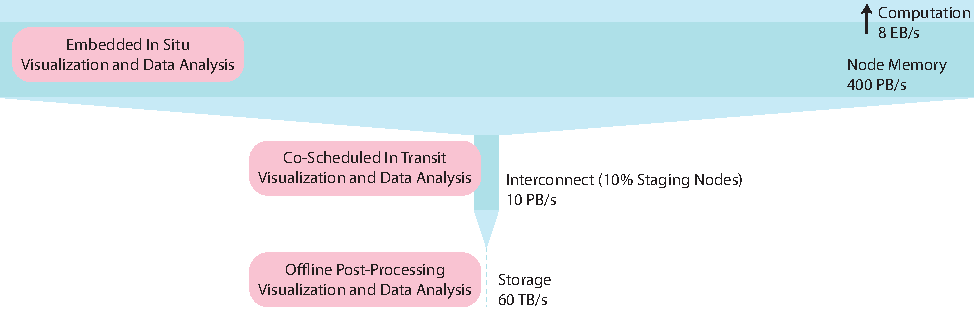
\includegraphics{figures/IOBandwidths}
  \caption[Relative bandwidth of exascale system components.]{Visual
    depiction of the relative bandwidth of exascale system components based
    on predictions of exascale
    machines\lcite{ScientificDiscoveryExascale2011,ExascaleArchitecturesReport}.}
  \label{fig:IOBandwidths}
\end{figure}

Figure~\ref{fig:IOBandwidths} provides a Minard plot depicting the
bandwidths of different I/O components by the proportional width of their
respective blue bars.  (See Tufte\scite{Tufte2001} for a longer description
of Minard plots and their merits.)  Not shown on this plot is the rate at
which data can be computed.  At $10^{18}$ double precision floating point
operations per second, the exascale computer on aggregate will produce 8~EB
per second.  On this plot that would be over 10 feet across.  The aggregate
bandwidth of the local memory --- that is, the speed at which data can be
pulled from memory to a local process summed over the entire machine --- is
400~PB/s.  This is as fast as we can reasonably expect to access data on
the system, but it is only available in the same job space as the running
simulation.  If we were to offload that data to another job, say a staging
job running on a generous allocation of 10\% of the overall nodes, then we
could stream the data to this job at 10~PB/s, which is pretty fast but only
2.5\% the local access rate.  Furthermore, one must worry about the limited
memory available on the staging nodes.  To move the data entirely to disk
storage, the bandwidth drops way down to 60~TB/s.  This is only 0.015\% the
rate at which data can be written to local memory and only 0.00075\% the
rate at which data can be computed.  So, only an extremely small fraction
of data can ever hope to be captured on disk.

Because there is such a disparity between computation rate and storage
bandwidth, \keyterm{\insitu visualization}, the visualization of data while
still present in the working memory of a simulation and before being
transferred to disk storage, features predominately in plans for near and
far term
\vda\lcite{ScientificDiscoveryExascale2011,VisualizationKnowledgeDiscovery2007,Childs2007,Moreland2012:Ultravis}.
An important consequence is the system wide implications resulting from the
solution to this problem, which include scientific domain specific analysis
techniques, \insitu framework development, and complexity impacts in
post-processing.

\fix{Dave originally had text arguing that another reason that data could
  not be saved to disk was the power cost.  However, I think the power cost
  is reflected in the bandwidth and capacity of the system.  Unless there
  is a further limitation of the system due to power, such as the peak
  bandwidth cannot be maintained due to power restrictions and will quickly
  be throttled back, or that there will be a measured cost added to
  projects to save more data, then I don't see the point of adding the
  extra detail.  I don't recall ever seeing any such predictions.}

\begin{figure}
  \centering
  \subfloat
      [Traditional offline post-processing \vda.]
      {
        
\includegraphics{figures/WorkflowsOffline}
        \label{fig:Workflows:Offline}
      } \\
  \subfloat
      [Embedded \insitu \vda (VDA).]
      {
        
\includegraphics{figures/WorkflowsInSitu}
        \label{fig:Workflows:InSitu}
      } \\
  \subfloat
      [Service-oriented \intransit \vda (VDA).]
      {
        
\includegraphics{figures/WorkflowsInTransit}
        \label{fig:Workflows:InTransit}
      }
  \caption[Visualization and data analysis workflows.]{Traditional and
    emerging workflow diagrams showing the flow of information from
    simulation to persistent storage.  In all cases data will later be
    retrieved from storage and further analyzed.}
  \label{fig:Workflows}
\end{figure}

Figure~\ref{fig:Workflows} shows simplified diagrams showing the flow of
information from simulation to persistent storage in a typical modeling and
simulation workflow.  Typical \vda occurs as an offline post-processing
step, after the simulation has written results directly to persistent
storage (Figure~\ref{fig:Workflows:Offline}).  Often, these results are in
a code-specific format, and are formatted as ``restart'' files ---
optimized for reading back into an instance of the science code, and not
optimized for post processing analysis by \vda tools.

Extreme computation size and extreme architectures force data flows like
those in Figures \ref{fig:Workflows:InSitu} and
\ref{fig:Workflows:InTransit} in which \vda is performed on the simulation
results before they are written to persistent storage.  In
Figure~\ref{fig:Workflows:InSitu}, data are handed directly to an
\keyterm{embedded \insitu} \vda library coupled with the running code,
enabling analysis, visualization and data reduction under the control of
the science code --- at the cost of sharing runtime resources with the \vda
execution.  In Figure~\ref{fig:Workflows:InTransit}, data are transferred
to an \keyterm{\intransit} \vda process separate from the running code.
This decouples the data computation and \vda processes, which affords many
advantages but at the cost of system complexity.  Both approaches must be
provided for extreme scale analysis, so that the codes, system designers,
and science customers can design a computation and analysis workflow suited
to the specific needs of the science, analysis, and decision process being
supported.

\subsection{Contributions}

To facilitate the transition to these new workflows, our group is
developing supporting technologies to help implement the tighter coupling
between simulation and \vda.  To this end we are contributing to two key
enabling projects: Catalyst and Nessie.

\keyterm{Catalyst} is an \insitu library that provides a simplified
interface to \vda through direct function calls.  The primary intention is
to provide a \vda service to simulation codes as demonstrated in the
workflow of Figure~\ref{fig:Workflows:InSitu}.  Catalyst is described in
more detail in Section~\ref{sec:Catalyst}.

\keyterm{Nessie} is an I/O service that provides remote-procedure call
abstractions and one-sided data-message passing.  Nessie makes
communication between parallel jobs more simple and efficient, and we use
it to facilitate the transfer of simulation data from simulation to \vda
service in the \intransit workflow of Figure~\ref{fig:Workflows:InTransit}.
Nessie is described in more detail in Section~\ref{sec:Nessie}.

With these tools we can implement the multiple workflows of
Figure~\ref{fig:Workflows} and compare their relative performance.  For
this comparison, we implement a use case, described in
Section~\ref{sec:UseCase}, which is representative of some real-world
problems being addressed by our users at Sandia National Laboratories.  The
results of these comparisons are given in Section~\ref{sec:Results}.


\section{Scope}
\label{sec:Scope}

\subsection{State of the Art}

When this Milestone was designed, there were three types of activities that addressed large scale data analysis: post-processing, code-specific in-situ solutions, and communication frameworks concerned with data movement.

Specialized solutions are specific instantiations of in-situ processing tuned for a particular code.  Examples include CTH's \fix{blar} and the \fix{other blar that Kwan Liu is developing with Jackie Chan}.  These are highly efficient in-situ analysis codes developed in tandem with a specific code, and represent the pathway to the most efficient in-situ solution, tuned for the data structures, the memory/compute time tradeoffs and analysis needs of a specific customer in a specific domain.  As such, we expect that specialized solutions will always offer the most compact, optimized in-situ processing for the codes they were designed for.  However, applying these in-situ codes to other domains and codes requires an investment in engineering (they cannot always be easily abstracted from the target code), a tradeoff in flexibility (they are often designed to achieve a specific analysis or visualization task, often one that lends itself to optimization at large scale), and a tradeoff in community support and engagement.

Another option for large scale in-situ analysis is to create a capability that is intended to support a large range of data types, analysis operations and visualization modes.  A generalized engineering solution would be more flexible, but perhaps less efficient than one tuned for a specific code.  This type of library would provide analysis capabilities for a range of problems, providing a method of prototyping and iterating on many types of analysis.  Valuable or common analysis operations can then be optimized as needed for specific codes.  This is the option that is at the core of our Milestone.

The value of this contribution is to promote the investigation of a larger tradeoff space, in which memory, compute time, analysis type, and storage can all be traded more flexibly to achieve a required analytics end.  By building a robust, cross-platform capability for large scale in-situ analysis, we hope to build a community that exercises different options in the tradeoff space, allowing analysts and scientists the capability to explore the impact of different combinations of memory, processing time, energy, storage, analysis algorithms to achieve their results.  In particular, as we continue towards larger, ever diverse computation platforms, it is beneficial to the community to invest in analysis capabilites that provide a range of options, so that tradeoff space can be easily explored.

Thus, this Milestone has promoted work on a common analysis library - Catalyst - that is now capable of scaling to ASC-sized coupled analysis runs.  A complimentary data movement capability - Nessie - was also developed to promote the tradeoff between types of in-situ analysis, and help explore the optimal solutions for resource allocation, data transport, and analytics processing.



\section{Official Milestone}
\label{sec:OfficialMilestone}

The following is the ASC milestone our work implements.

\begin{quotation}

ASC calculations produce complex datasets that are increasingly difficult to explore and understand using traditional post-processing workflows.  To advance understanding of underlying physics, uncertainties, and results of ASC codes, SNL must gather as much relevant data as possible from large simulations.  This drives SNL to couple data analysis and visualization capability with a running simulation, so that high fidelity data can be extracted and written to disk.  This Milestone evaluates two approaches for providing such a coupling:

\begin{enumerate}
\begin{item}
In-situ processing provides ``tightly-coupled'' analysis capabilities through libraries linked directly with the simulation.  SNL has collaborated on developing an in-situ capability designed for this purpose.
\end{item}
\begin{item}
In-transit processing provides ``loosely-coupled'' analysis capabilities by performing the analysis on separate processing resources.  SNL provides this capability through a ``data services'' capability designed for this purpose.
\end{item}
\end{enumerate}

SNL will engineer, test and evaluate customer-driven operations on large-scale data created by a running simulation.  The data operations will be performed by instrumented versions of both the in-situ and in-transit solutions, with the resulting performance data published and made available to the ASC community.

A program review will be conducted, and its results documented.  A report will be submitted as a record of milestone completion.

\end{quotation}

The approaches described in the milestone correspond to the workflows in
Figure~\ref{fig:Workflows:InSitu} and Figure~\ref{fig:Workflows:InTransit},
respectively.  As previously described, we implement these two approaches
using Catalyst and Nessie.

Our ``customer-driven operations'' are encapsulated in the use case given
in Section~\ref{sec:UseCase}, which was provided by Jason Wilke to 
represent a typical shock physics analysis.

The results of our instrumentation on the coupled simulation and \vda are
given in Section~\ref{sec:Results}.  These results come from experimental
runs on the Cielo supercomputer\lcite{Doerfler2011} ranging up to over 64
thousand cores.  Our measurements record the cost of coupling \vda to a
running simulation in terms of added execution time and memory overhead,
which satisfies the deliverables of the milestone.


\section{Catalyst}
\label{sec:Catalyst}

Although it is straightforward for a simulation development team to add some
basic \vda capabilities into simulation code, our desire is to have a
general-purpose fully-featured library that leverages existing
implementations.  The intention is threefold.  First, by leveraging existing
\vda libraries we can benefit from the accumulation of over two decades of
visualization research and development.  Second, by making the library
general purpose we can quickly apply our \insitu \vda capabilities to many
simulations as opposed to a single simulation.  Third, by using our
existing code we can integrate the \insitu tools with our traditional
post-processing tools both to provide interfaces that users are already
familiar and comfortable with and to apply scalable algorithms designed for
\insitu with our post-processing tools and vice versa.

Catalyst is a C++ library with an externally facing API to C, FORTRAN, and
Python.  It is built atop the Visualization Toolkit (VTK)\lcite{VTK} and
ParaView\lcite{ParaView}.  By building Catalyst with VTK, it can access a
large number of algorithms including writers for I/O, rendering algorithms,
and processing algorithms such as isosurface extraction, slicing, and flow
particle tracking.  Catalyst uses ParaView to implement and manage the
\vda, which is defined using a visualization
pipeline\lcite{Moreland2013:TVCG}.  Although it is possible to construct
pipelines entirely in C++, the ParaView control structure allows pipelines
configured through Python scripts.

\begin{figure}[htb]
  \centering
  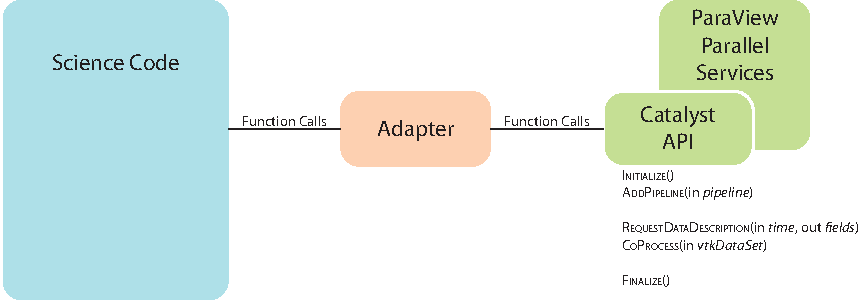
\includegraphics{figures/CatalystCoupling}
  \caption{Coupling a simulation with Catalyst.}
  \label{fig:CatalystCoupling}
\end{figure}

\subsection{Catalyst Architecture}

Catalyst boils the ParaView and VTK architecture down into five API calls that
manage all the processing required for operating a processing pipeline.
Initialize and Finalize are expected calls when dealing with MPI; this is where
Catalyst will first access MPI World.  RequestDataDescription and CoProcess
handle the hand-shake from the simulation code to Catalyst.
RequestDataDescription passed current time information to Catalyst, and
Catalyst passes back whether or not it should process and which fields it
needs.  This may allow the simulation code, through the adaptor described
below, to efficiently pass only what is necessary at that time.  The CoProcess
call is where control is passed to Catalyst for processing.  This call will
hang until Catalyst finishes and returns control to the simulation.

The AddPipeline call is where a majority of the work is done.  Although there
is usually only one pipeline object passed to Catalyst, it is possible to pass
several.  It is also common for this pipeline object to be written in Python
because this is the native scripting language for ParaView, but it is possible
for the pipeline to be hard coded C++.  While there is some overhead cost to
using Python code in the pipeline here, it is very low due to its nature as a
glue code combining the C++ filters which are written in VTK.  The advantage is
that the scripted pipeline can change to access any feature available in
Catalyst while only compiling the capability once.

\begin{figure}[htb]
  \centering
  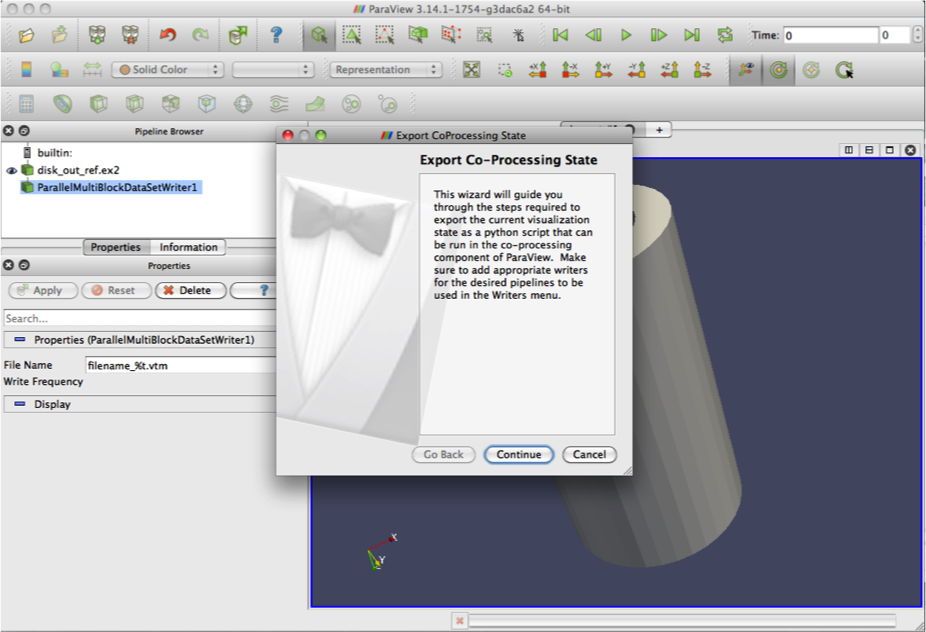
\includegraphics{figures/ScriptExport}
  \caption{Wizard plugin within ParaView to export interactive traces as 
Catalyst pipelines for use within a coupled simulation.}
  \label{fig:ScriptExport}
\end{figure}

In addition to the advantages of writing Python pipeline scripts by hand, there
is a well supported plugin for ParaView that will automatically create Catalyst
Python scripts automatically from within the GUI, based on traces of user
interaction with the GUI, Figure~\ref{fig:ScriptExport}.  This plugin works by
replacing a file read at the top of the pipeline with the same VTK data object
provided by the adaptor (described below).  From the perspective of the
pipeline it could be operating on data being read from a file, but this data is
coming from an in-memory \insitu transfer.  The plugin will examine all views
currently open within the ParaView view and create equivalent views with
independent image sizes in the script.  It is also possible to make place-holder
objects within the pipeline to act as file write points.  Usually these will be
placed at the end of a long chain of processing to store the resulting
processed data, but it is also possible to splice these file writes earler in
the pipeline to see the effects of different stages of processing.  Each file
and image writer can write at an independent frequency, allowing for very
infrequent writes of potentially large files while also allowing for more
frequent small image writes as the simulation proceeds.

\subsection{Simulation Adaptor}

Since Catalyst will extend to a variety of existing simulation codes, our
design does not expect its API to easily and efficiently process internal
structures in all possible codes directly.  Our solution is to rely on
adapters --- which are small pieces of code written for each new linked
simulation --- to translate data structures between the simulation's code
(for our use case the CTH shock physics code) and Catalyst's VTK-based
architecture, as shown in Figure~\ref{fig:CatalystCoupling}.  The adapter
must also establish a mechanism that allows the simulation to define a
visualization pipeline and periodically invoke the analysis while running
the simulation, which in our CTH adapter we control through the CTH input
deck.

To conserve memory, our adapter directly interfaces the \vda code to the
data structures defined by CTH.  This interface is challenging because
although the blocks of data are represented sequentially in both CTH and
VTK, the multidimensional order is different.  To address this, our adapter
contains an interface wrapper above the standard VTK array.  The wrapper
reimplements the array's accessor functions to handle the order difference
between the two systems.  Although there is a minor overhead in additional
pointer arithmetic and virtual method calls, it saves us from a deep memory
copy.

\subsection{References}

The Catalyst library and the algorithms we use within CTH are an
accumulation of several years work, starting with the development of
fragment analysis algorithms with our post-processing
tools\lcite{Moreland2008:UltraVis,Ice2009,Moreland2010}, described in more
detail in Section~\ref{sec:UseCase}.  Subsequent work lead to the
development of Catalyst\lcite{Fabian2011} and the scaling of algorithms
used in conjunction with CTH\lcite{Fabian2012}.


\section{Nessie}
\label{sec:Nessie}

\fix{Ron}

\fix{Description}

\fix{Why Nessie (why not ADIOS?)}


\section{Use Case}
\label{sec:UseCase}

\fix{Nathan}

For the purposes of this milestone, we explore the problem of
characterizing fragments in an explosion simulation.  Simulation is a vital
part in understanding shock physics.  Although experimentation will always
be a necessary tool for scientific inquiry and corroboration, the amount of
data we can retrieve with experimentation is limited.  Experiments in shock
physics usually involve high energy, high velocities, and high variability,
all of which hinder detailed, accurate, and repeatable observations during
the experiment.  When measurements cannot be taken during the experiment,
they must be taken after the experiment by observing the remaining
material.  Much can be learned in the manner, but the transient states
during the experiment are lost.

Another limiting factor of experimentation is its high cost and slow
turnaround.  To create shock physics experiments, physical devices must be
fabricated.  These devices are then usually destroyed during the
experiment.  Safety and political issues also often plague shock physics
experiments.  In some cases, experimentation is simply not feasible.  Thus,
simulation plays a major role in shock physics analysis.

In this milestone, we use an example simulation of an exploding pipe shown
in Figure~\ref{fig:ExplodingPipe}.  This similation problem is provided to
our group by Jason Wilke.  In addition to well representing the kinds of
simulation and analysis done at Sandia National Laboratories, this
simulation provides interesting results and many different levels of
refinement, which allows us to scale the problem from less than 100 cores
to well over 10,000 cores.

\begin{figure}[htb]
  \centering
  \framebox[\linewidth]{Images of exploding pipe, \`{a} la Figure 2 in
    Nathan's LDAV paper.}
  \caption{Simulation of an exploding pipe, which presents many
    prototypical fragment analysis challenges.}
  \label{fig:ExplodingPipe}
\end{figure}

One of the most important features in shock physics analysis is material
fragments.  The physical properties of the fragments, including mass,
volume, and shape, as well as their trajectories, can all be important.  In
particular, shape can be an important characteristic.  Consider the example
fragments given in Figure~\ref{fig:Fragments}.  The top fragment is long
and sharp, making it more likely to penetrate objects.  In comparison, the
bottom left fragment is rounded and could have less damage potential.
However, the U-shaped fragment in the bottom right may be harmful depending
on the scenario, but could be difficult to distinguish from the round
fragment in many shape metrics.

\begin{figure}[htb]
  \centering
  \framebox[\linewidth]{Example fragments, \`{a} la Figure 1 in Nathan's
    LDAV paper.}
  \caption{Examples of potential fragments that we would like to
    characterize.}
  \label{fig:Fragments}
\end{figure}

The simulation code we use is CTH\lcite{CTH,CTHAMR}.  It is an Eulerian
shock physics code that uses an adaptive mesh refinement (AMR) data model.
These adaptive finite volumes can take up different amounts of space
depending on where they are in the model and how closely the simulation is
refining the space.

In order to correctly find fragments, we must first determine what is and
is not a fragment.  The simulation operates on a finite volume and
comprises a set of simulated materials, which each take up a certain
fraction of finite cells within that volume.  We treat any connected region
of cells with material volume fraction above a given threshold as a
fragment of that material.  Generally speaking, when a simulation begins,
each material comprises usually one connected region, which we refer to as
the main mass.  As the simulation progresses, this region breaks apart and
gaps occur between pieces of material, filled either by another material or
by the surrounding air.  Once there is a gap as wide as at least one cell,
we determine that a fragment as formed.  The challenge when finding these
fragments on a large scale parallel system is that regions that make up the
fragments straddle process boundaries, requiring communication between the
processes to determine the full shape of a fragment.

Because the number of fragments a shock physics simulation can generate are
so numerous, it is seldom realistic for a person to examine every one.  It
is therefore more beneficial to first perform computational analytics that
provide useful summary statistics and identify particularly interesting
fragments.  This analysis has the added benefit of reducing the amount of
memory required to represent it.  Therefore, fragment analysis is a good
candidate for \insitu processing.

A full fragment analysis requires multiple steps.
\begin{enumerate}
\item Identify the boundaries of fragments.  This transition over the
  volume fraction threshold allows us to separate what is and is not a
  fragment.
\item Find the fragment connected components.  A connected components
  analysis brings together all finite elements that belong to a single
  fragment.
\item Characterize properties of fragments.  Given the collected elements
  for each fragment, find the features such as shape volume, and movement
  that are of interest.
\item Extract useful information.  This could involve, for example,
  computing histograms of features or extracting a small subset of
  fragments deemed important.
\end{enumerate}

\emph{For the purpose of simplifying the problem and making it tractable
  for analysis, we abbreviate the problem to include only the
  identification of fragment boundaries} for the results of this milestone.
The creation of fragment boundaries is a nontrivial problem in that we must
make sure the surface is ``watertight'' in that the representative mesh
surface is conforming and closed.  Making a surface from an AMR mesh
watertight is challenging because the AMR mesh itself is nonconforming at
boundaries between adjacent regions at different levels of refinement.

\begin{figure}[htb]
  \centering
  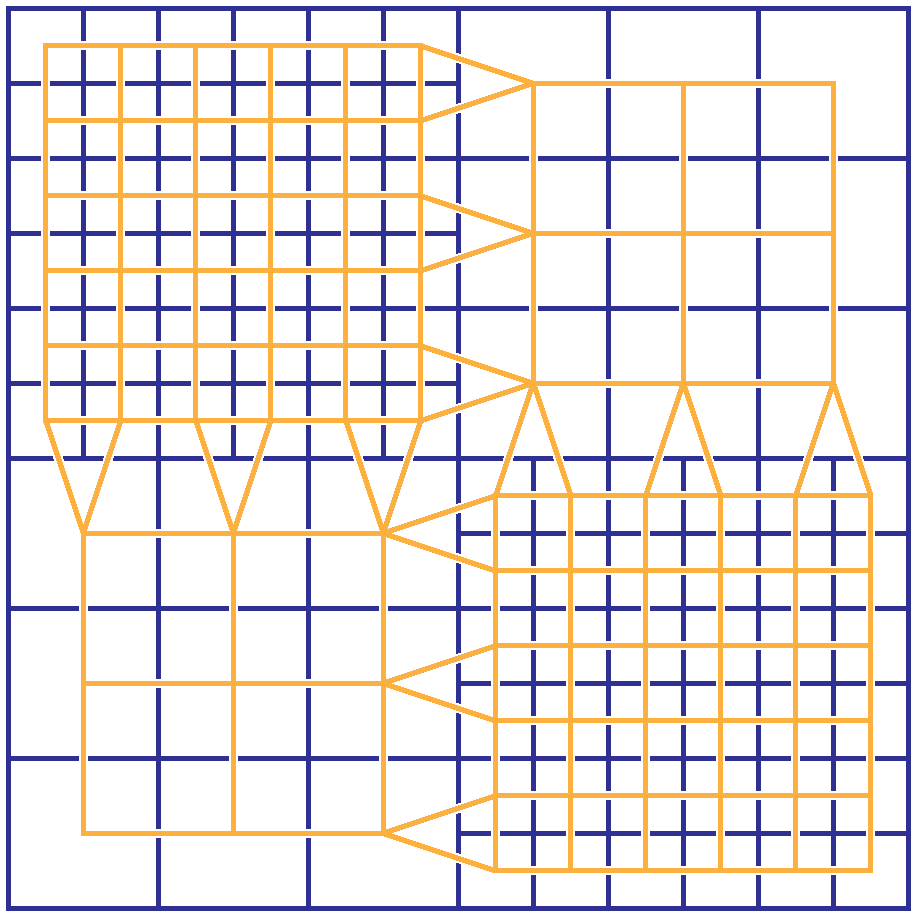
\includegraphics[width=5in]{figures/AMRDual}
  \caption{A simple 2D AMR example with 2 different refinement levels (blue
    lines) and the conforming dual grid we build with it (yellow lines).}
  \label{fig:AMRDual}
\end{figure}

To generate this watertight fragment surface, we first build a dual mesh of
the original AMR mesh.  The dual mesh contains a vertex at the center of
each cell in the original mesh and an edge through each face of of the
original mesh as demonstrated in Figure~\ref{fig:AMRDual}.  The advantage
of creating a dual mesh is that it is straightforward to build conforming
cells across the boundaries of AMR regions with different levels of
refinement.

The disadvantage of building these dual meshes in a distributed parallel
job is that neighborhood information must be shared between regions that
might be located on different processes.  Resolving this neighborhood
information requires a significant amount of communication.  (Such
communication would be necessary for any creation of a watertight mesh.)
This communication can limit the scalability of the algorithm.

Efficient communication of boundary elements first requires that each
process knows the location of the neighbors for each region it holds.  If
data is loaded with no knowledge of its decomposition, which is typical in
the post-processing of data, then this neighborhood information can be
retrieved only through global communication.  Our initial
\keyterm{baseline} algorithm starts with this global communication, which
we find to severely limit the scalability of the algorithm.

However, when running the surface creation algorithm as an embedded \insitu
component of CTH, this global communication of finding neighbors is
wasteful because CTH already has this information.  To take advantage of
this neighborhood information, we make a small change to CTH to pass this
data decomposition information through its I/O layer to Catalyst.  With
this data, our \keyterm{refined} algorithm skips the global communication
leaving only the more scalable boundary-data passing.  Our analysis shows
that the refined algorithm is much more scalable than the baseline
algorithm\lcite{Fabian2012}.  Unfortunately, we cannot apply the refined
algorithm in the \intransit workflow because this workflow redistributes
the data and invalidates this neighborhood information from CTH.


\section{Results}
\label{sec:Results}

\fix{Nathan and Ron}

\begin{figure}[htb]
  \centering
  \includegraphics[width=\linewidth]{figures/MemoryUsageInSituPerNode.pdf}
  \caption{Plot of average per node memory usage of the in-situ run on Cielo.}
  \label{fig:MemoryInSituPerNode}
\end{figure}

\begin{figure}[htb]
  \centering
  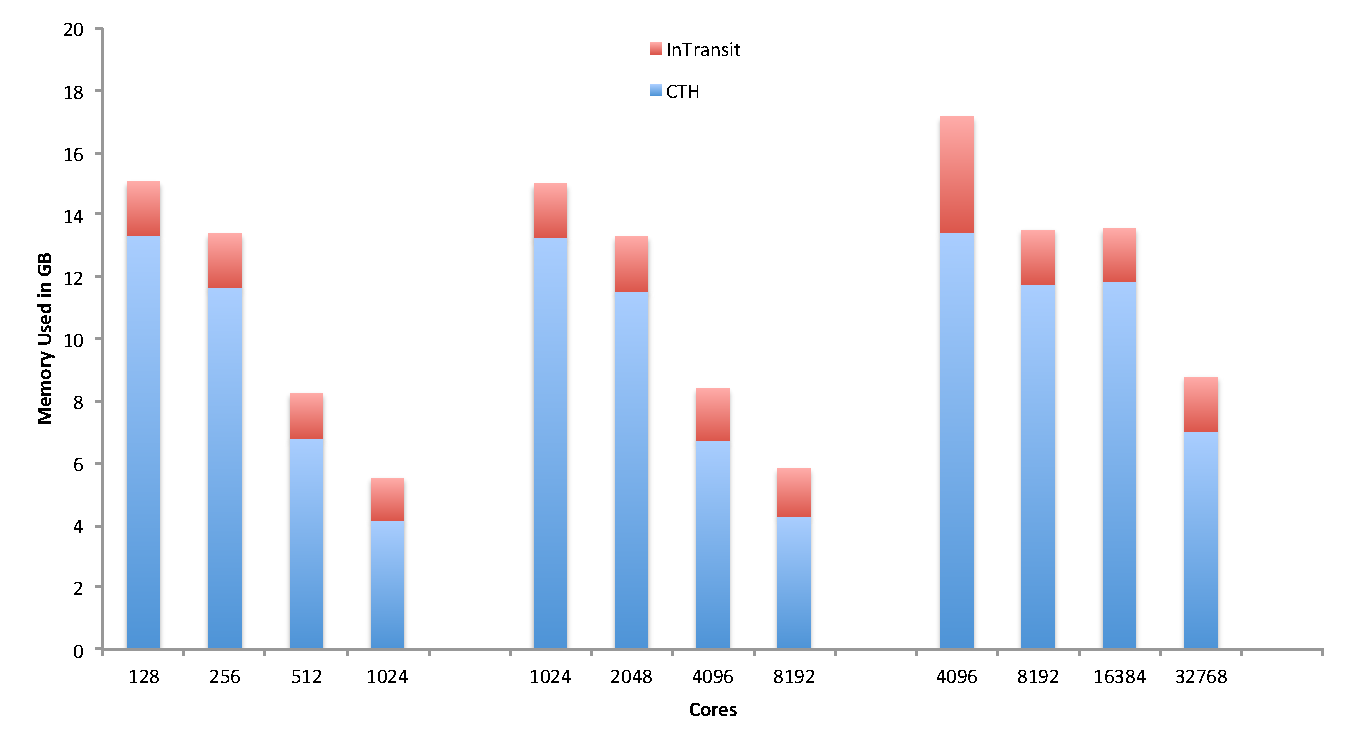
\includegraphics[width=\linewidth]{figures/MemoryUsageInTransitPerNode.pdf}
  \caption{Plot of average per node memory usage of the in-transit run on Cielo.}
  \label{fig:MemoryInTransitPerNode}
\end{figure}

\begin{figure}[htb]
  \centering
  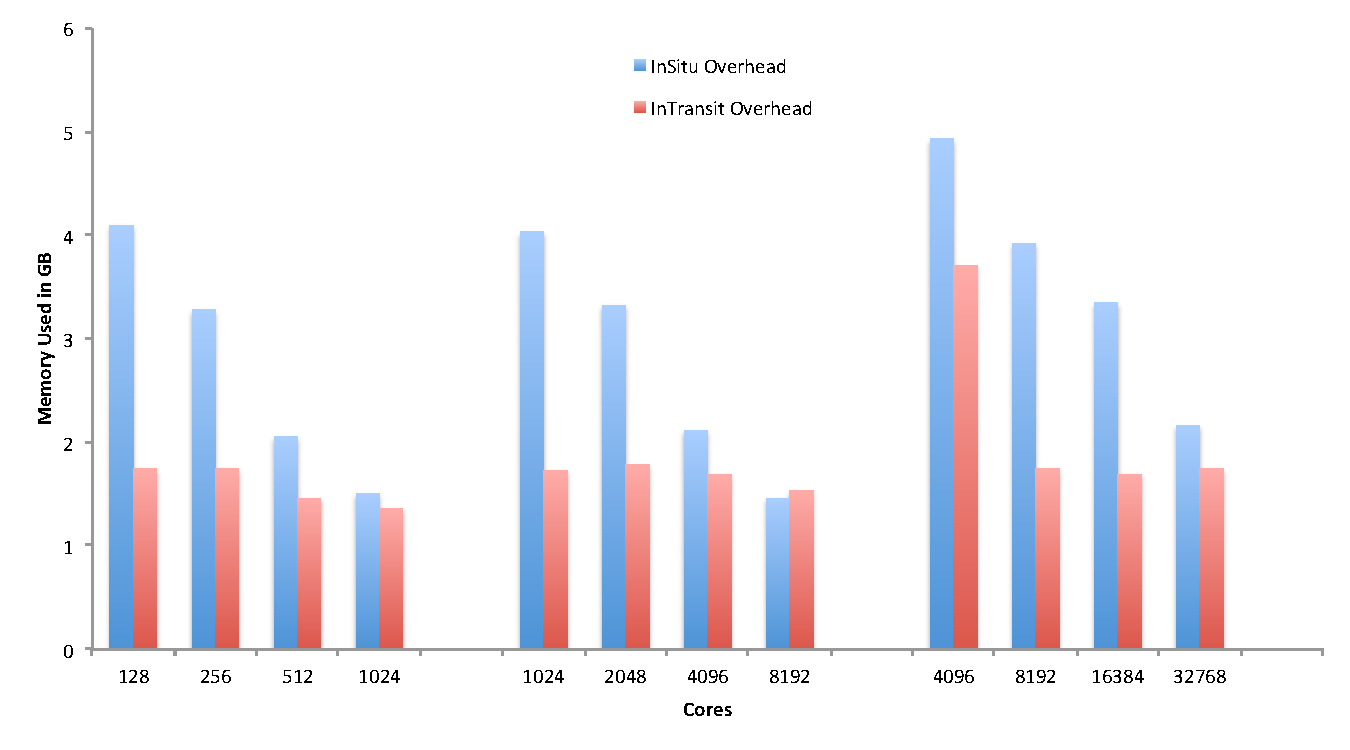
\includegraphics[width=\linewidth]{figures/MemoryUsageCompare.pdf}
  \caption{Plot of the average overhead per node of both InSitu and InTransit}
  \label{fig:MemoryCompare}
\end{figure}

\begin{figure}[htb]
  \centering
  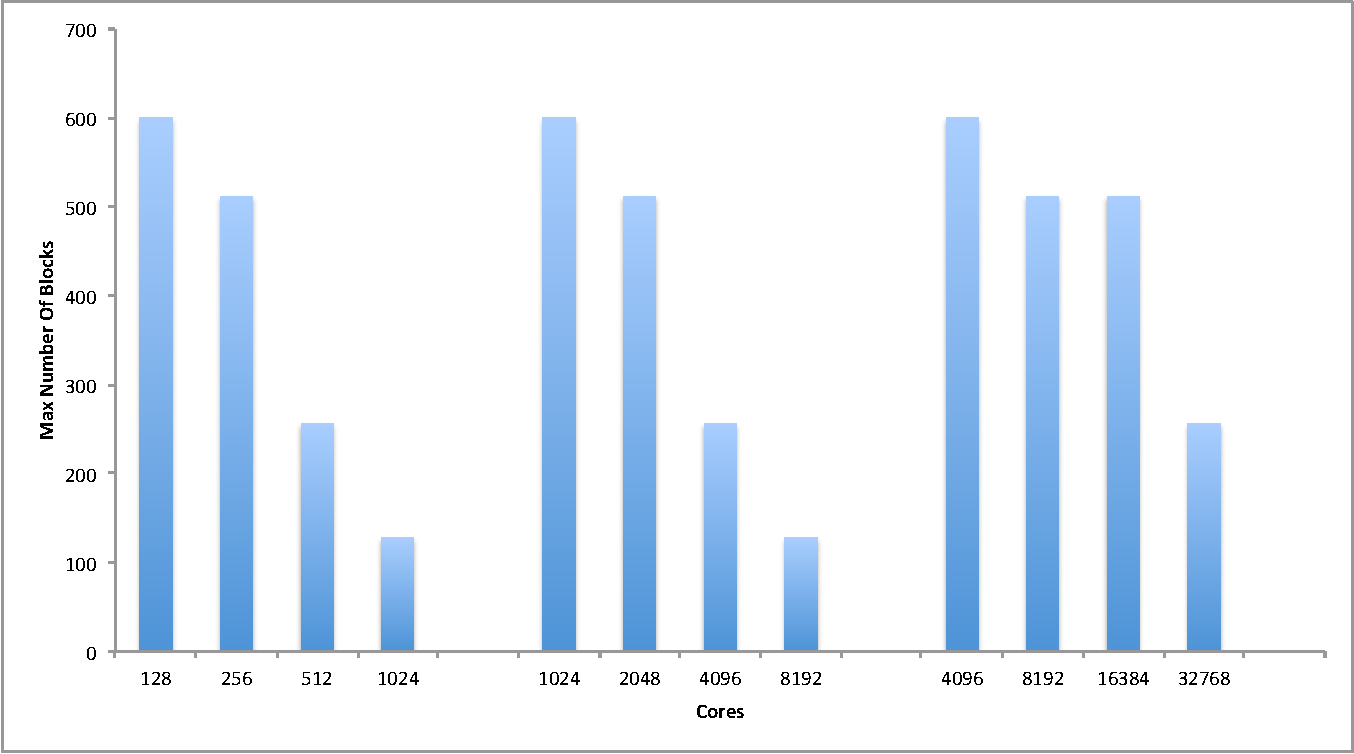
\includegraphics[width=\linewidth]{figures/MaxNumberOfBlocks.pdf}
  \caption{A plot of the "max number of blocks" parameter supplied to CTH for each run.}
  \label{fig:MaxBlocks}
\end{figure}

In order to under the CTH memory sizes, it is important to note that CTH
preallocates memory based on a value for "max number of blocks" provided
through the input deck.  Because of this, CTH memory usage is highly impacted
by the user specification.  In this case we ran the results with what we
believe are reasonable values for "max number of blocks" given the size of the
problem.  Figure~\ref{fig:MaxBlocks} shows the corresponding max blocks for
each run.




\section{Conclusions}
\label{sec:Conclusion}

This document summarizes a significant scaling study resulting from over 9
million core-hours of execution and analyzes the comparative performance of
multiple workflows for performing \vda on simulation results.  Most of
these workflows benefit from running in tandem with the simulation to
analyze its transient data before it is written to storage.  Based on this
analysis, we make the following conclusions.

\paragraph{\Intransit can provide a performance improvement over \insitu in
  some circumstances, but the window is narrower than we anticipated.}  
\Intransit analysis has an added overhead above embedded
\insitu analysis involving transferring data between parallel jobs.  Given
an analysis with perfect linear scalability, we suspect \intransit
workflows will always have an added cost, and our results support this.
With an analysis that does not scale perfectly, possibly due to
communication overhead, it is theoretically possible for \intransit to be
faster by reducing the size of the analysis job.  This is one of the
motivations for choosing an analysis task that requires significant
communication.  In our results, we do find instances where \intransit is
faster, but by a smaller margin and for fewer configurations than we
initially anticipated.  So although \intransit has several other positive
features, we do not anticipate performance to be the main motivations for
using it.

\paragraph{Memory overhead will be an important trade-off space.}
The baseline amount of memory added to the CTH job to perform \insitu
processing is roughly 100MB per core.  Considering that our embedded
\insitu library is a fully featured visualization toolkit containing over 2
million lines of code and algorithms developed over almost 2 decades, this
overhead is not unreasonable.  Nevertheless, this footprint can be
problematic for simulations already tight on memory.  Because of this,
efforts are already underway to improve our memory footprint by making
finer modules and being more selective on the available algorithms.  This,
of course, requires a compromise between the size of the library and the
algorithms that are dynamically available.  We also note that our algorithm
has the potential to generate sizable meshes of its own.  Thus, it may be
fruitful to pursue and support incremental algorithms where possible.

\paragraph{Initialization time matters.}  Our scaling efforts to date
focus on the scalability of the algorithms invoked during the run of a
simulation.  The initialization cost, a one-time penalty, has yet to be
seriously considered.  However, based on our HPCToolkit measurements,
initialization becomes a significant cost at high process counts.

\paragraph{Disk-based I/O is not dead\ldots{} yet.} Our initial assumption
was that it would not be feasible to output full results at a fine enough
temporal resolution from CTH to disk storage to perform our high fidelity
analysis.  However, our control workflow shows that although the overall
time to write data to disk and then read back again incurs a large cost, it
is still realistic to do so.  Thus, users may still choose to incur the
extra overhead to use a traditional offline post-processing \vda workflow.

\paragraph{Better job scheduling is important.} One of the more complicated
parts of running an \intransit workflow is scheduling the simulation job
and service job to run in tandem.  Frankly, the capabilities of the
scheduler are inadequate for our needs.  We cannot start and stop jobs
independently and make reconnections dynamically.  Another experiment we
would like to do but is challenging to schedule is to allow simulation and
service to share nodes.  Since each node has 16 cores, perhaps we could get
better transfer performance by allocating one core per node for service and
the rest for simulation.  A similar scheduling scheme will be important to
take advantage of burst buffers in future architectures.

\fix{Timeline of work ahead.}



% ---------------------------------------------------------------------- %
% References
%
\clearpage
% If hyperref is included, then \phantomsection is already defined.
% If not, we need to define it.
\providecommand*{\phantomsection}{}
\phantomsection
\addcontentsline{toc}{section}{References}
\bibliographystyle{plain}
\bibliography{MilestoneFY13}


% ---------------------------------------------------------------------- %
%
\appendix

\section{Signed Letter from Committee}

\section{Executive Summary Slides}

\section{Raw Data}

% \printindex

%
% Some distributions are required by Sandia; e.g. the housekeeping copies.
% Depending on the type of report; e.g. CRADA, Patent Caution, etc.
% additional distribution lines may have to be added. See the "Guide for
% Preparing SAND Reports"
%
% SANDdistribution takes CA or NM as an optional argument. If given,
% the approrpiate housekeeping copies are inserted autmatically.
% Inside the SANDdistribution environment, several commands can be used
% insert the distributions for CRADA, LDRD, etc. See example below.
%
% You can leave the CA or NM option off and not use any of the SANDdist*
% commands. This will allow you to create a distribution list manually.
%
\begin{SANDdistribution}[NM]

  % Some external Addresses
  \SANDdistExternal{1}{James Ahrens\\ Los Alamos National Laboratory\\ P.O. Box 1663\\ Los Alamos, NM 87545}
  \SANDdistExternal{1}{Berk Geveci\\ Kitware, Inc.\\ 28 Corporate Drive\\ Clifton Park, NY 12065}
  \SANDdistExternal{1}{Lucy Nowell\\ U.S. Department of Energy\\ SC-21\\ 19901 Germantown Road\\ Germantown, MD 20874-1290}
  \SANDdistExternal{1}{Becky Springmeyer\\ Lawrence Livermore National Laboratory MS 555\\ P.O Box 808\\ 7000 East Ave.\\ Livermore, CA 94551}

  \bigskip


  % Internal Addresses
  \SANDdistInternal{1}{1319}{Ronald Brightwell}{01423}
  \SANDdistInternal{1}{0380}{Micheal Glass}{01545}
  \SANDdistInternal{1}{1319}{Suzanne Kelly}{01423}
  \SANDdistInternal{1}{0380}{Kyran Mish}{01542}
  \SANDdistInternal{1}{0823}{Constantine Pavlakos}{09326}
  \SANDdistInternal{1}{0380}{Kendall Pierson}{01542}
  \SANDdistInternal{1}{0783}{Jason Wilke}{06634}

  \SANDdistInternal{2}{1326}{Nathan Fabian}{01461}
  \SANDdistInternal{2}{1326}{Kenneth Moreland}{01461}
  \SANDdistInternal{2}{1319}{Ron Oldfield}{01423}
  \SANDdistInternal{2}{1326}{David Rogers}{01461}

\end{SANDdistribution}



% The second printing
%\begin{SANDreDistribution}
%    \SANDdistExternal{}{}
%    \bigskip
%    \SANDdistInternal{}{}{}{}
%    \SANDdistInternalM{}{}{}{}
%\end{SANDreDistribution}

\end{document}
